% arara: pdflatex: { synctex: yes }
% arara: makeindex: { style: ctuthesis }
%% arara: bibtex

%\listfiles


%\PassOptionsToPackage{cp1250}{inputenc}

% The class takes all the key=value arguments that \ctusetup does,
% and couple more: draft and oneside
\documentclass[twoside]{ctuthesis}

\makeatletter
\edef\mytoday{\expandafter\@gobbletwo\the\year\ifnum\month<10 0\fi\the\month\ifnum\day<10 0\fi\the\day}
\makeatother

% LaTeX logo with better kerning in sf bf font
\makeatletter
\newcommand\LaTeX@lmss@bx{L\kern -.33em{\sbox \z@ T\vbox to\ht \z@ {\hbox {\check@mathfonts \fontsize \sf@size \z@ \math@fontsfalse \selectfont A}\vss }}\kern -.15em\TeX}
\DeclareRobustCommand\myLaTeX{%
	\ifcsname LaTeX@\f@family @\f@series\endcsname
		\csname LaTeX@\f@family @\f@series\endcsname
	\else
		\LaTeX
	\fi
}

\ctusetup{
%	preprint = {\ctuverlog \\ ctuman \mytoday},
	mainlanguage = czech,
	titlelanguage = czech,
	otherlanguages = {english, czech},
	title-czech = {Následování člověka mobilním robotem},
	title-english = {},
	doctype-czech = {Bakalářská práce},
	doctype-english = {},
	xfaculty = F3,
	department-czech = {Katedra kybernetiky},
	department-english = {Department of Cybernetics},
	author = {Mykhaylo Zelenskyy},
	supervisor = {Ing. Jan Chudoba},
%	supervisor-address = {Ústav X, \\ Uliční 5, \\ Praha 99},
	keywords-czech = {manuál, závěrečnná práce, \LaTeX},
	keywords-english = {manual, degree project, \LaTeX},
	day = 25,
	month = 3,
	year = 2017,
%	list-of-figures = false,
%	list-of-tables = false,
%	monochrome = true,
%	savetoner = true,
	pkg-listings = true,
	ctulstbg = none,
%	layout-short = true,
%	pkg-hyperref = false,
}

\ctuprocess

% Theorem declarations, this is the reasonable default, anybody can do what they wish.
% If you prefer theorems in italics rather than slanted, use \theoremstyle{plainit}
\theoremstyle{plain}
\newtheorem{theorem}{Theorem}[chapter]
\newtheorem{corollary}[theorem]{Corollary}
\newtheorem{lemma}[theorem]{Lemma}
\newtheorem{proposition}[theorem]{Proposition}

\theoremstyle{definition}
\newtheorem{definition}[theorem]{Definition}
\newtheorem{example}[theorem]{Example}
\newtheorem{conjecture}[theorem]{Conjecture}

\theoremstyle{note}
\newtheorem*{remark*}{Remark}
\newtheorem{remark}[theorem]{Remark}

\DeclareMathOperator{\atantwo}{atan2}

% Marginpars used as navigation aids.
\usepackage{mparhack}
\usepackage{epstopdf}
\usepackage{subfig}
\usepackage{siunitx}


\newcommand\indexmp[1]{{\sffamily\bfseries#1}}

\ExplSyntaxOn
\cs_new:Nn \ctuman_domarginpar:n {
	\marginpar
	[ \raggedleft \footnotesize \sffamily #1 ]
	{ \raggedright \footnotesize \sffamily #1 }
}
\cs_generate_variant:Nn \ctuman_domarginpar:n { x }
\DeclareDocumentCommand \ctump { m } {
	\clist_set:Nn \ctuman_temp_clist { #1 }
	\ctuman_domarginpar:x { \clist_use:Nnnn \ctuman_temp_clist { \\ } { \\ } { \\ } }
	\clist_map_inline:Nn \ctuman_temp_clist { \index{##1|indexmp} }
	\ignorespaces
}
\ExplSyntaxOff

% Abstract in Czech
\begin{abstract-czech}
Tento mánuál představuje \LaTeX ovou třídu ctuthesis, její použití, požadavky na systém atd.
\end{abstract-czech}

% Abstract in English
\begin{abstract-english}
This manual shows how to use the ctuthesis \LaTeX\ class, what are the requirements, etc.
\end{abstract-english}

% Acknowledgements / Podekovani
\begin{thanks}
Chtěl bych poděkovat svému vedoucímu, Ing. Janu Chudobovi, za jeho rady a nápady. 
\end{thanks}

% Declaration / Prohlaseni
\begin{declaration}
I declare that this work is all my own work and I have cited all sources I have
used in the bibliography.

\medskip

Prague, \monthinlanguage{second} \ctufield{day}, \ctufield{year}

\vspace*{2cm}

Prohlašuji, že jsem předloženou práci vypracoval samostatně, a že jsem uvedl veškerou použitou literaturu.

\medskip

V Praze, \ctufield{day}.~\monthinlanguage{title}~\ctufield{year}
\end{declaration}

\usepackage{url}

\usepackage{tabularx,array}

\usepackage{mathtools,amssymb}

% A savebox for typesetting listings in the titles
\newsavebox{\myboxa}

%\newcommand*\symbO{$\color{red}\bowtie$}
\newcommand*\symbO{\raisebox{0.5\height}{\scalebox{0.7}{\color{red}${\vartriangleright}\mkern-6mu{\vartriangleleft}$}}}
\newcommand*\symbM{\raisebox{0.5\height}{\scalebox{0.7}{\color{red}${\blacktriangleright}\mkern-6mu{\blacktriangleleft}$}}}
\newcommand*\itemO{\item\leavevmode\kern-0.33em\symbO}
\newcommand*\itemM{\item\leavevmode\kern-0.33em\symbM}



\begin{document}
	


% We actually don't want inline listings to have a background color
\renewcommand \ctulstsep {0pt}

% \ctuclsname for typesetting the class' name
\newcommand\ctuclsname{\leavevmode\unhcopy\ctuclsnamebox}
\newsavebox\ctuclsnamebox
\begin{lrbox}{\ctuclsnamebox}
\ctulst!ctuthesis!
\end{lrbox}

\maketitle

\chapter{Úvod}

Pomocný robot může se zdát mnoha z nás jako futuristický sen. Takový robot, který by místo nás nosil věci, pomáhal při nákupech, asistoval v nemocnicích nebo ošetřoval raněné ve válkách. Podobný robot by měl tolik výhod, že by v budoucnu to bylo trendem vlastnit takového pomocníka.

Bylo provedeno hodně různých výzkumů ohledně návrhu robotu, který by dokázal sledoval člověka. S tímto problémem jsou spojené dvě důležité otázky. První je jaké senzory použit pro lokalizaci člověka, druhá řeší řízení a navigaci robotu, aby udržoval určitou vzdálenost a vyhýbal se případným překážkám.

Nejdříve je třeba definovat, co vlastně je robot následující člověka. Jedná se o mobilního robota, který sleduje určitou osobu
a zároveň objíždí překážky a chová se k ostatním lidem, jako k překážkám, tj. nezmění cíl sledování během jízdy.

Takový robot typicky může být vybaven hodně různými senzory, např. laserovým, zvukovým nebo IČ dálkoměrem, aby mohl měřit vzdálenost od překážek, kamerou pro detekci sledovaného objektu, bezdrátovým přenášečem signálu, GPS apod. Tyto senzory by měly fungovat současně, aby robot dokázal všechno, co se od něj očekává. 

\section{Cíl práce}
Cílem této práce je navrhnout systém pro řízení robotu, aby dokázal sledovat člověka a vyhýbat se překážkám. Jelikož cíl pro robota by měl být unikátní, použije se vizuální značka, která by tento problém měla vyřešit. Robot dopředu bude vědět, jaký typ značky musí hledat, tím pádem se snižuje šance, že si splete cíl s jiným člověkem nebo překážkou.

Při návrhu tohoto systému je třeba uvědomit si několik věcí:
\begin{enumerate}
	\item Cíl se nesmí pohybovat větší rychlostí, než je maximální rychlost robotu. Může se stát, že robot už nikdy nedokáže najít sledovaného člověka, dokud se dotyčný nevrátí na dostatečně blízkou k robotu pozici.
	
	\item Aby značka byla dobře detekovatelná, musí být umístěna v ochranném prostředí, tj. být kontrastní v porovnání s pozadím.
	
	\item V případě použití dálkoměru pro měření vzdálenosti mezi objekty, je důležité, aby systém nedetekoval sledovaný cíl jako překážku.
\end{enumerate}

\section{Motivace}

Jak již bylo řečeno, robot s podobnou funkcionalitou by byl hodně užitečný nejen jako pomocník v každodenní činnosti lidí. V medicínských zařízených a domovech pro seniory takový robota by se mohl starat o pacienty (viz \ref{rnc}), také by našel své uplatnění v armádě, kde by pomáhal vojákům s různými náklady. Určitě vylepšená varianta robota následujícího člověka by mohla posloužit jako tělesná stráž.


\begin{figure}
	\caption{Robot následující člověka}
	
	\label{rnc}
	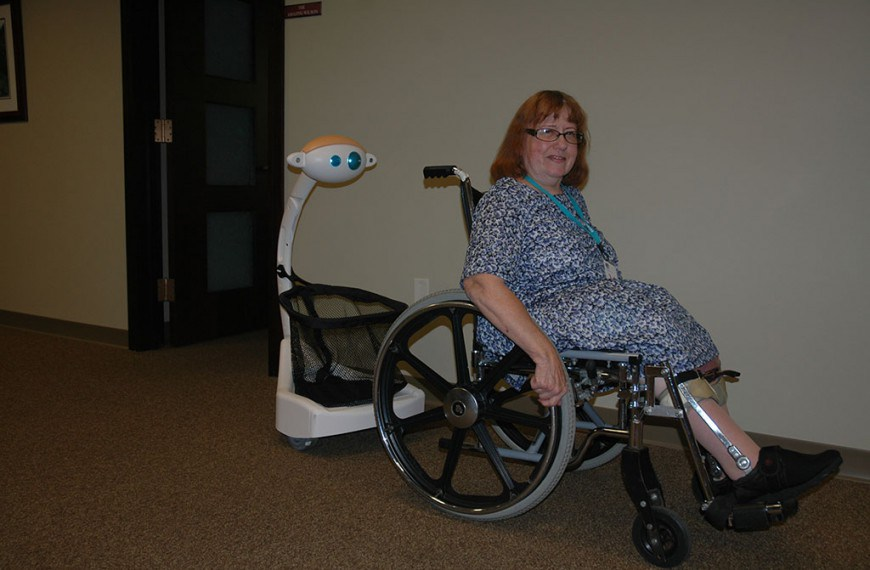
\includegraphics[width=\textwidth]{images/0/maxresdefault.jpg}
\end{figure}



\chapter{Návrh systému}
\section{Volba vizuální značky}
%https://www.researchgate.net/publication/270107591_Visual_Localization_of_Mobile_Robot_Using_Artificial_Markers
%https://pdfs.semanticscholar.org/71e8/30b6da4b7adbfcd369664e5347a515e25d64.pdf
%http://www.uco.es/investiga/grupos/ava/sites/default/files/GarridoJurado2014.pdf
Jak již bylo zmíněno, mobilní robot bude následovat člověka, který má na sobě umístěnou předem známou vizuální značku. Pro tyto účely se v praxi běžně používají markery pro rozšířenou realitu. Jejich detekce je většinou jednoduchá a můžou v sobě uchovávat užitečnou informaci, např. identifikační číslo, podle kterého robot pozná, koho sleduje. Jednu z možných vizuálních značek, které jsou použity v práci, lze vidět na obrázku \ref{am}.

\begin{figure}[H]
	\caption{Příklad vizuální značky}
	
	\label{am}
	
\includegraphics[width=0.5\textwidth]{images/2/ArucoMarker.jpg}
\end{figure}

\section{Volba souřadnicového systému}
\label{ss_section}

Pro řízení robotu je třeba zvolit souřadnicový systém, ve kterém se bude pohybovat. 

Počátek zvolené souřadnicové soustavy je umístěn do počáteční pozice robotu a osy X je ve stejném směru, jako počáteční směr jízdy robotu. Kladný směr jízdy robotu je v kladném směru osy Y, jak je vyobrazeno na \ref{ss}, a je v rozmezí $\left(-\pi; \pi\right)$. Poloha cíle (viz sekci \ref{mereni_polohy_cile}) je potom vztažená k poloze robotu a je počítána v čárkované soustavě, jejíž počátek je umístěn do aktuální pozice robotu, a je vůči původní otočená o $h$, kde $h$ je směr jízdy robotu.

\begin{figure}[H]
	\caption{Použitý souřadnicový systém}
	
	\label{ss}
	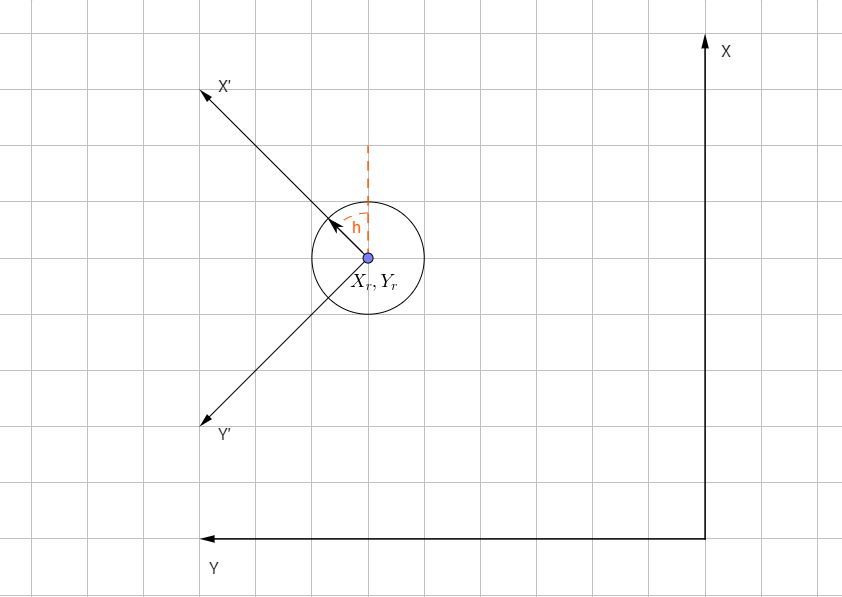
\includegraphics[width=0.9\textwidth]{images/2/ss.png}
\end{figure}

\section{Implementační záležitosti}

%http://opencv.org/about.html
%https://www.uco.es/investiga/grupos/ava/node/26
Protože se očekává, že software, který bude výsledkem této práce, bude běžet real-time, musí být rychlý a stabilní. Z těchto důvodů bylo rozhodnuto, že celá implementace bude udělána v jazyce C++.

Kromě toho pro C++ je vytvořená OpenCV knihovna, která nabízí obrovské možnosti pro práci s obrazem. Tato knihovna obsahuje přes 2500 optimalizovaných algoritmů pro počítačové vidění a strojové učení. Některé z nich budou použity pro detekci vizuální značky ve výstupu z kamery. Navíc v této knihovně je implementován algoritmus pro detekci ArUco markeru, který je podrobněji popsán v sekci \ref{aruco_marker}.

\chapter{Detekce}

\section{Zpracování obrazu z kamery}

Než bude možné použít rozpoznávací algoritmy, výstup z kamery musí být náležitě zpracován, aby odpovídal formátu, se kterým algoritmy pracují.

% http://citeseerx.ist.psu.edu/viewdoc/download?doi=10.1.1.420.7883&rep=rep1&type=pdf
%http://docs.opencv.org/trunk/d9/d8b/tutorial_py_contours_hierarchy.html
%http://docs.opencv.org/3.1.0/d5/dae/tutorial_aruco_detection.html
%https://en.wikipedia.org/wiki/Ramer–Douglas–Peucker_algorithm#cite_ref-1
Načtený snímek je převeden do černobílé podoby, je tedy použito prahování. Jelikož se předpokládá, že se robot může pohybovat v prostředí s nerovnoměrným osvětlením, pro binarizaci obrazu je vhodné použit adaptivní prahování \ref{adapt}. Tato metoda počítá práh pro malé části obrazu místo globálního nastavení prahu pro celý snímek.

Dále je třeba najít kontury. Algoritmus pro nalezení kontur je implementován v OpenCV knihovně. Tato funkce navíc zajišťuje zachování hierarchii kontur, tedy topologii obrázku, jako je vidět na \ref{hierarch}. Tato informace je užitečné pro následující rozpoznávání, protože pak kontury na nejnižší nebo nejvyšší úrovni hierarchie můžou být ignorovány, pokud se předpokládá, že vizuální značka bude umístěna v ochranné zóně a bude obsahovat další pod-vzory.

\begin{figure}
	\caption{Příklad použití adaptivního prahování}
	
	\label{adapt}
	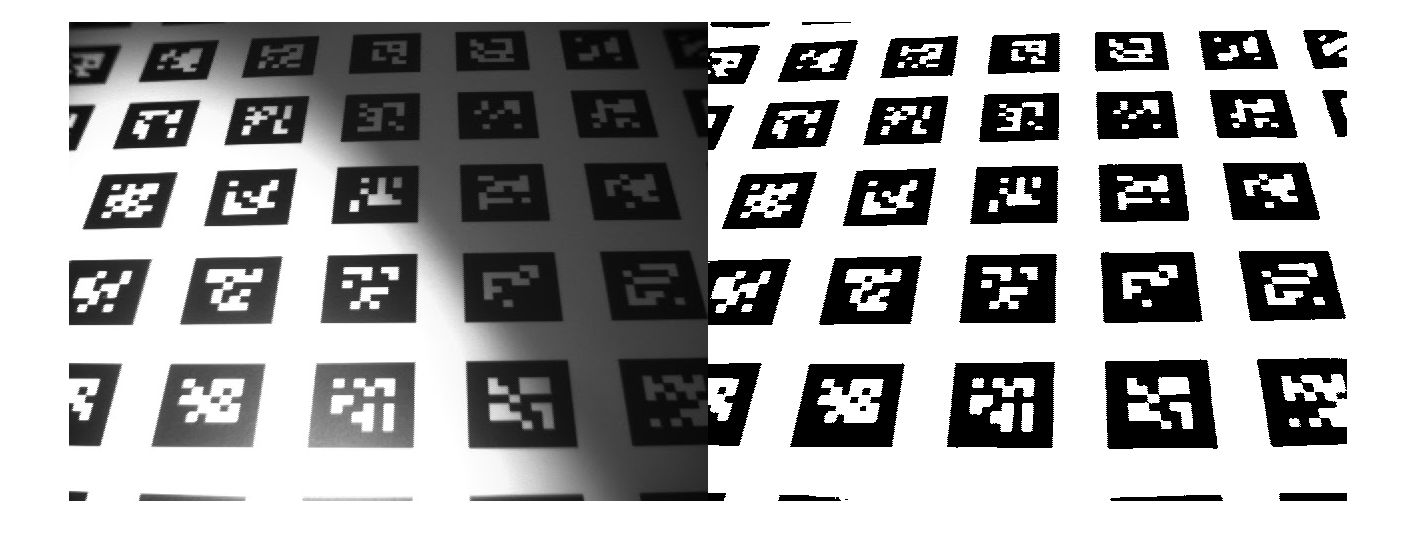
\includegraphics[width=0.8\textwidth]{images/2/adapt.jpg}
\end{figure}

\begin{figure}
	
	\caption{Hierarchie (topologie) obrazu}
	
	\label{hierarch}
	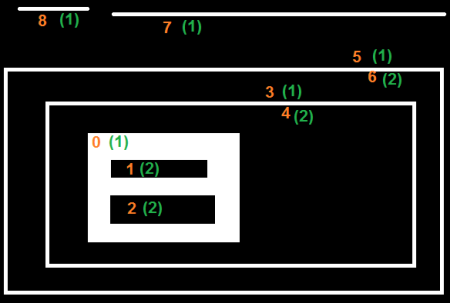
\includegraphics[width=0.8\textwidth]{images/2/ccomp_hierarchy.png}
\end{figure}

\section{Rozpoznávání vzoru}

Pro rozpoznávání vizuální značky byly zvoleny dva algoritmy: jeden založený na korelaci známých vzorů s nalezeným, druhý přímo z OpenCV knihovny -- ArUco marker detektor.

\subsection{Korelační algoritmus}

Tento algoritmus využívá principu korelaci mezi dvěma veličinami, tedy mezi známým vzorem a nalezenou oblasti zájmu (Region of Interest, ROI). Korelace uvádí, jak jsou na sobě tyto veličiny závislé, a může nabývat hodnot od -1 do +1. Hodnota korelačního koeficientu blížící se -1 značí nepřímou závislost veličin, koeficient blízký +1 naopak značí přímou závislost, což je zobrazeno na \ref{korelace}.

\begin{figure}
	
	\caption{Příklad korelace mezi dvěma veličinami}
	
	\label{korelace}	
	\subfloat[Kladná korelace]{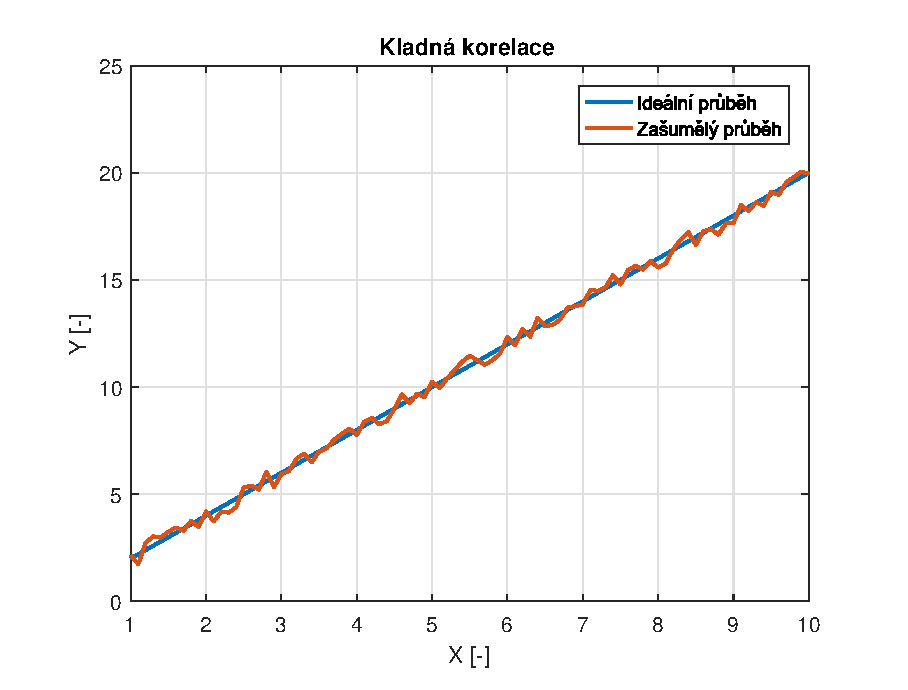
\includegraphics[width=0.5\textwidth]{images/2/klad.eps}}
	\subfloat[Záporná korelace]{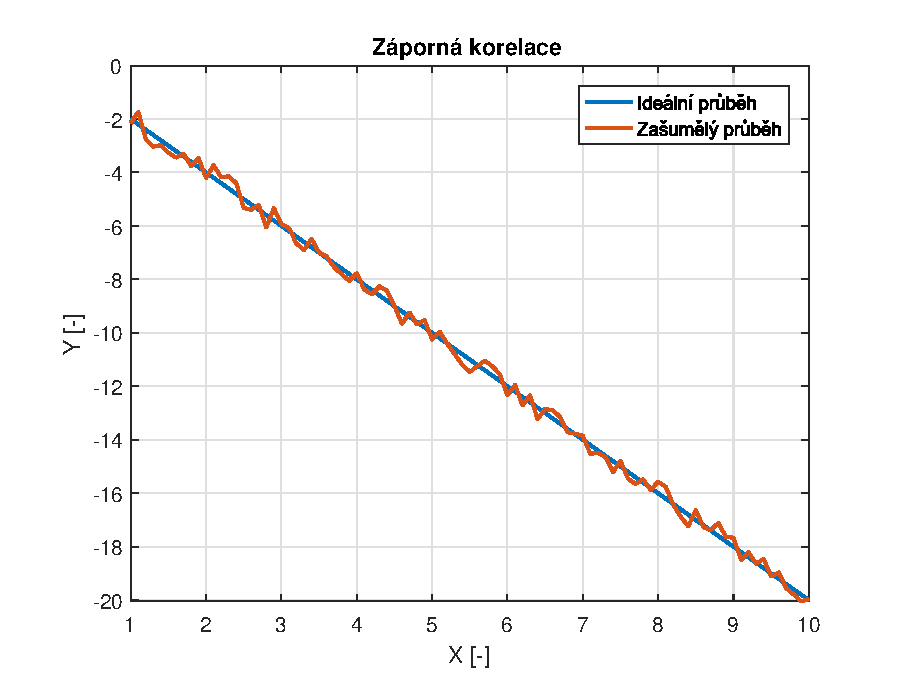
\includegraphics[width=0.5\textwidth]{images/2/zap.eps}}
	\hfill
	\subfloat[Žádná korelace]{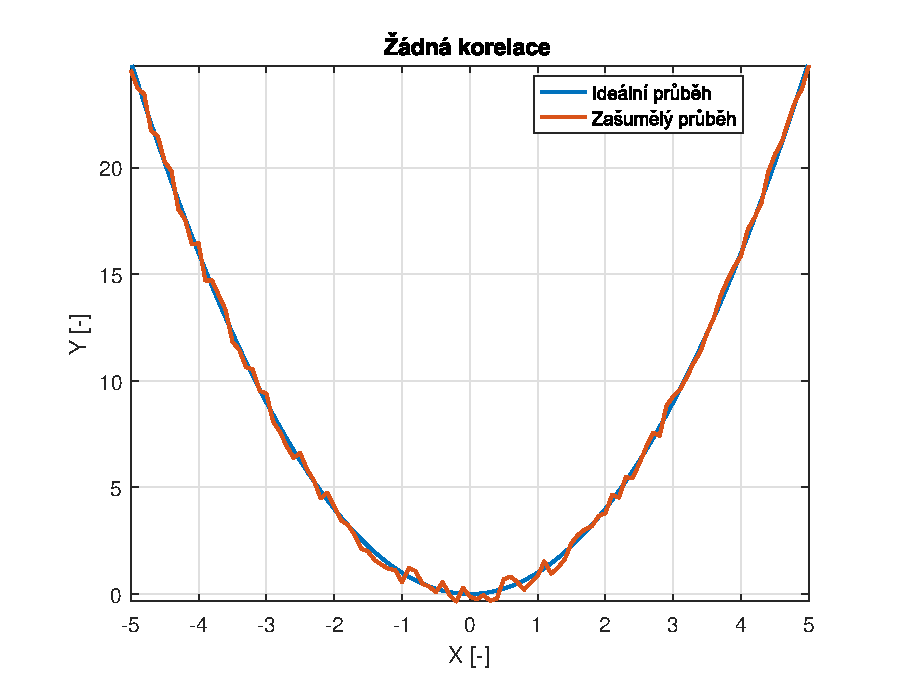
\includegraphics[width=0.5\textwidth]{images/2/zadna.eps}}
\end{figure}
Hledaná ROI v zjednodušeném případě je konvexní čtyřúhelník, proto stačí s použitím informace o topologii obrazu spočítat polygony nalezených kontur a vybrat pouze ty, co obsahují čtyři strany a nejsou konkávní. Pro aproximaci křivky se používá Ramerův Douglasův Peuckerův algoritmus (viz \ref{approx}), který je naimplementován v OpenCV knihovně.
\begin{figure}
	
	\caption{Aproximace křivky pomocí Ramerova Douglasova Peuckerova algoritmu}
	
	\label{approx}
	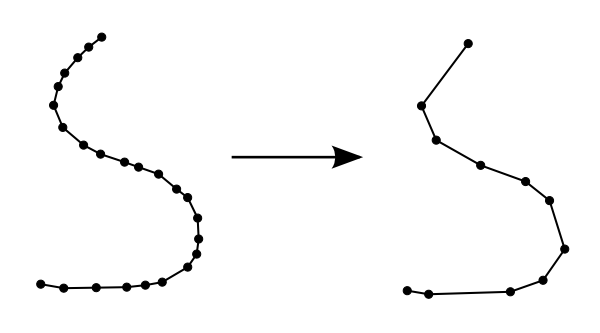
\includegraphics[width=0.8\textwidth]{images/2/approx.png}
\end{figure}


Následně je spočítána transformační matice mezi nalezeným polygonem a známým vzorem. Pomocí této matice se polygon převede do takové podoby, aby byl porovnatelný se vzorem.

Dále se jenom vyhodnotí, jak nalezená ROI a známý vzor jsou na sobě závislý. Pokud je vypočtený korelační koeficient větší, než zadaný práh, ROI se vyhodnotí jako správně označena a algoritmus vrátí souřadnice jejích rohů pro následující zpracování.

Korelaci mezi dvěma obrázky $I_1$ a $I_2$ s $N$ pixely spočítáme následujícím způsobem:

	\begin{equation}
	\mu_{1,2} = \frac{\sum_{i,j}I_{i,j}}{N},
	\end{equation}
	\begin{equation}
	\sigma_{1,2} = \sqrt{\left(\frac{\sum_{i,j}(I_{i,j} - \mu_{1,2})^2}{N}\right)^2},
	\end{equation}
	\begin{equation}
	covar(I_1, I_2) = \frac{(I_1 - \mu_1)\cdot(I_2 - \mu_2)}{N},
	\end{equation}	
	\begin{equation}
	cor(I_1, I_2) = \frac{covar(I_1, I_2)}{\sigma_1 \sigma_2}.
	\end{equation}
	
\subsection{ArUco marker detektor}
\label{aruco_marker}
	
Tento algoritmus je naimplementován v OpenCV knihovně a umožňuje rozpoznávání ArUco markerů nebo podobných vizuálních značek. Podobně jako výše uvedený korelační algoritmus, hledá konvexní čtyřúhelník. Rozdíl pak spočívá v odlišném zpracování nalezené ROI, kde se místo korelace využívá binární mapa kandidáta.

ROI je rozdělena na mřížku s počtem buněk rovným počtu bitů hledaného vzoru (viz \ref{cell}). Následně se spočítá, kolik bílých a černých pixelů obsahuje každá buňka, na základě čehož se vyhodnotí, jestli buňka je černá nebo bílá (viz \ref{cellm}). Pokud detektor ve svém slovníku obsahuje vzor se stejnou binární maskou, vrátí souřadnice rohů nalezené ROI.

\begin{figure}
	\caption{Buňky ArUco markeru}
	
	\label{cell}
	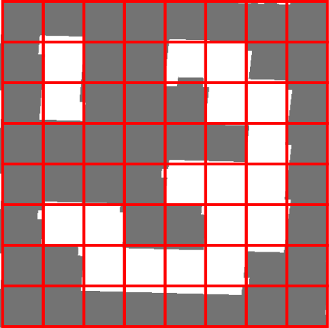
\includegraphics[width=0.5\textwidth]{images/2/bitsextraction1.png}
\end{figure}
\begin{figure}
	\caption{Vyhodnocení obrázku pomocí ArUco detektoru}
	
	\label{cellm}
	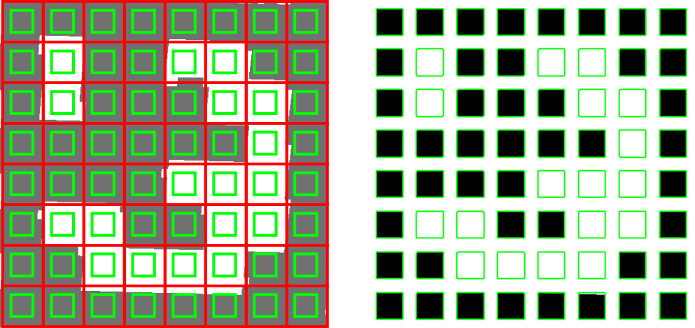
\includegraphics[width=1\textwidth]{images/2/bitsextraction2.png}
\end{figure}
\section{Měření polohy cíle}
\label{mereni_polohy_cile}
%http://www.huecandela.com/hue-x/pin-pdf/Prober-%20Wellman.pdf
Algoritmy popsané výše naleznou polohu vizuální značky v obraze, z čehož lze spočítat její umístění vůči kameře, je-li známa velikost této značky. Pro výpočty lze použít model ideální (dírkové) kamery, kde vzdálenost mezi kamerou a značkou je vyjádřena jako

\begin{equation}
d = \frac{fX}{x},
\end{equation}

kde

$x$: Nejkratší vzdálenost mezi dvěma rohy nalezené značky.

$f$: Ohnisková vzdálenost.

$X$: Známá délka hrany značky.

Pro nalezení posunutí značky vůči kameře při odklonění od její osy, musí být znám zorný úhel kamery. Ten lze spočítat dle vztahu

\begin{equation}
\alpha = 2\arctan\left(\frac{w}{2f}\right),
\end{equation}

kde

$w$: Šířka výstupního obrazu z kamery.

Potom úhel, který pokrývá jeden pixel snímku, je vyjádřen vztahem

\begin{equation}
APP = \frac{\alpha}{w}.
\end{equation}

Následně posunutí objektu vůči středu kamery je 

\begin{equation}
\phi = (x_c - x_t)APP,
\end{equation}

kde 

$x_c$: Pixel vyjadřující střed kamery v horizontálním směru.

$x_t$: Pixel vyjadřující střed nalezené značky v horizontálním směru.

\begin{figure}
	\caption{Měřené veličiny $d$ a $\phi$}
	
	\label{mereni}
	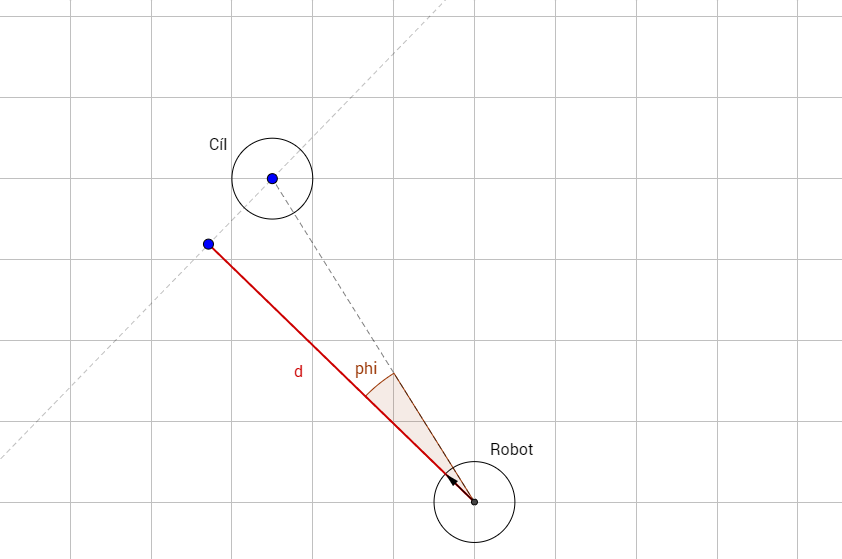
\includegraphics[width=1\textwidth]{images/2/mereni.png}
\end{figure}
\section{Kalmanův filtr}
\label{kalman_section}
%http://www.diss.fu-berlin.de/docs/servlets/MCRFileNodeServlet/FUDOCS_derivate_000000000473/2005_12.pdf
%https://github.com/rlabbe/Kalman-and-Bayesian-Filters-in-Python
V případě, že poloha značky vůči kameře není detekovatelná, robot by neměl zastavovat. Z tohoto důvodu je třeba predikovat polohu cíle z předchozích měření. Pro tyto účely v práci je použit Kalmanův filtr. 

Model lze popsat pomocí následujícího stavového vektoru
\begin{equation}
{\boldsymbol{x}} = 
\begin{bmatrix}
x&y&v_{x}&v_{y}
\end{bmatrix}^T,
\end{equation}

kde $v_{x}$, resp. $v_{y}$, značí rychlost ve směru osy X, resp. Y.


Stavový model je pak vyjádřen jako

\begin{equation}
\label{x_t+1}
{\boldsymbol{x}}_{t+1} = \boldsymbol{F}{\boldsymbol{x}}_{t},
\end{equation}

kde $\boldsymbol{F}$ je matice přechodu stavů $\boldsymbol{x}$ z času $t$ do času $t + 1$ a platí, že

\begin{equation}
\boldsymbol{F} = \begin{bmatrix}
1&0&1&0\\
0&1&0&1\\
0&0&dt&0\\
0&0&0&dt
\end{bmatrix}.
\end{equation}

Pro sledování cíle lze Kalmanův filtr rozdělit do tří kroků:

\textbf{1.  Inicializace ($t = 0$).} Během tohoto kroků se nastavuje počáteční pozice cíle $\boldsymbol{x}_0$ a výchozí hodnota pro kovarianční matici $\boldsymbol{P}_0$. Jelikož počáteční pozice cíle nemusí být známa, je vhodné zvolit $\boldsymbol{x}_0$ tak, aby v případě, že kamera nedetekuje značku po první iteraci, robot zůstával na místě.

\textbf{2. Predikce ($t > 0$).} V tomto kroku se provádí predikce polohy cíle v čase $t + 1$, tj. $\boldsymbol{x}_{t+1}$, dle \ref{x_t+1}. Také se počítá nová kovarianční matice dle následujícího vztahu

\begin{equation}	
\boldsymbol{P}_{t+1} = \boldsymbol{F}\boldsymbol{P}_t\boldsymbol{F}^T + \boldsymbol{Q}_{t+1},
\end{equation}

kde $\boldsymbol{Q}$ značí matici kovariancí šumů.

\textbf{3. Filtrace ($t > 0$).} Během tohoto kroku poloha cíle je upřesněna na základě provedeného měření. Nejdříve se spočte rozdíl mezi reálnou polohou a predikovanou v kroku 2.:

\begin{equation}
\boldsymbol{y}_{t} = \begin{bmatrix}
x_{m_t}\\y_{m_t}
\end{bmatrix} - \boldsymbol{H}\boldsymbol{x}_t,
\end{equation}

kde 

\begin{equation}
\boldsymbol{H} = \begin{bmatrix}
1&0&0&0\\
0&1&0&0
\end{bmatrix}.
\end{equation}

Dále se vypočítá Kalmanovo zesílení, pro nějž platí, že

\begin{equation}
\boldsymbol{K}_t = \boldsymbol{P}_t\boldsymbol{H}^T(\boldsymbol{H}\boldsymbol{P}_t\boldsymbol{H}^T + \boldsymbol{R})^{-1},
\end{equation}

kde $\boldsymbol{R}$ ja matice kovariancí šumů.

Následně se provede zpřesnění polohy cíle a aktualizuje se kovarianční matice:

\begin{equation}
\boldsymbol{x}_{t+1} = \boldsymbol{x}_t + \boldsymbol{K}_t\boldsymbol{y}_t,
\end{equation}

\begin{equation}	
\boldsymbol{P}_{t+1} = (\boldsymbol{I} - \boldsymbol{K}_t\boldsymbol{H})\boldsymbol{P}_t.
\end{equation}
\begin{figure}
	\caption{Shrnutí algoritmu Kalmanova filtru}
	
	\label{kalman_diag}
	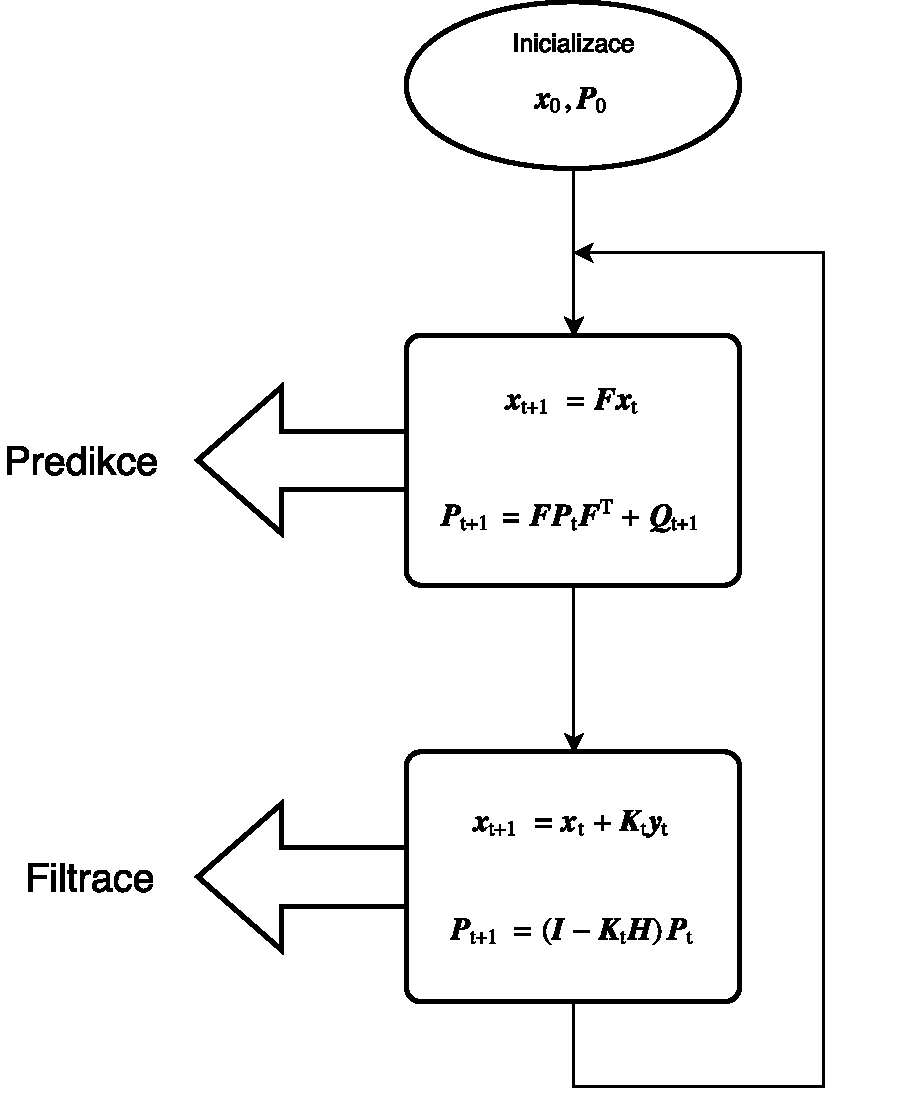
\includegraphics[width=0.9\textwidth, height=0.9\textwidth]{images/2/kalman_diagram.pdf}
\end{figure}
Z nalezených hodnot $x$ a $y$ lze jednoduše odvodit hodnoty $d$ a $\phi$, což je také vidět na \ref{inv}. Jelikož se předpokládá, že poloha robotu je známa, lze spočítat $x_t$ a $y_t$, což je poloha cíle vůči robotu, jako

\begin{equation}
x_t = x - x_r,
\end{equation}

\begin{equation}
y_t = y - y_r.
\end{equation}

Dále pak $\phi$ a $d$ jsou nalezeny dle vztahů

\begin{equation}
\phi = h - \atantwo(y_t, x_t),
\end{equation}

\begin{equation}
d = \sqrt{x_t + y_t}\cos(\phi).
\end{equation}
\begin{figure}
	\caption{Odvození hodnot $d$ a $\phi$ ze známé polohy cíle}
	
	\label{inv}
	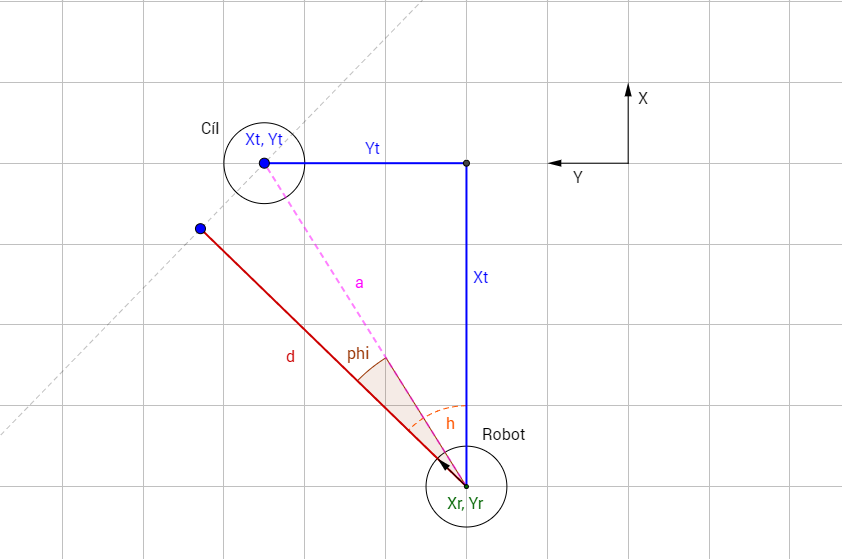
\includegraphics[width=1\textwidth]{images/2/neco.png}
\end{figure}
\chapter{Řízení robotu}

\section{Obstacle avoidance}

Pro řízení autonomního robotu je důležité, aby se dokázal vyhýbat překážkám, když sleduje svůj cíl. 

\subsection{Vector Field Histogram}

%http://www-personal.umich.edu/~johannb/Papers/paper16.pdf

%http://www.imavs.org/papers/2016/62_IMAV2016_Proceedings.pdf

Princip tohoto algoritmu spočívá v tom, že se na základě naměřených dat z dálkoměru vytvoří lokální mřížková mapa prostředí o poloměru $r_{map}$. Každá buňka této mapy tak obsahuje hodnotu obsazenosti odpovídající oblasti v reálném světě (viz \ref{mrizka}). Z této mapy se následně spočítá polární histogram, podle kterého se určí směr jízdy robotu.

\begin{figure}
	\caption{Lokální mapa prostředí o poloměru $r_{map}$ = 10}
	
	\label{mrizka}
	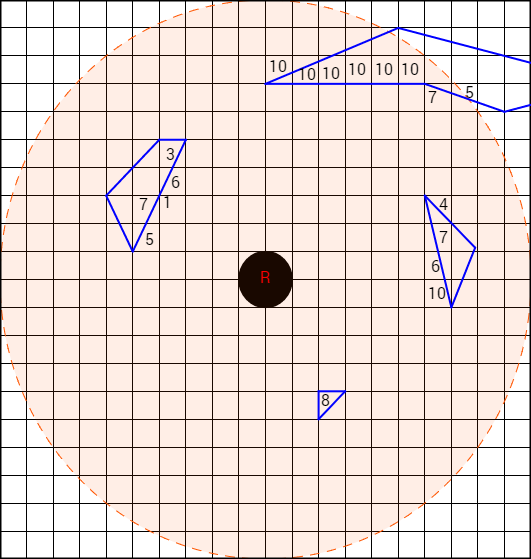
\includegraphics[width=0.6\textwidth, height = 0.6\textwidth]{images/3/mrizka.png}
\end{figure}

Celý proces tímto způsobem můžeme rozdělit na tři kroky: vytvoření primárního polárního histogramu, prahování primárního histogramu a vytvoření z něj binárního a výběr kandidátů pro směr pohybu.

\subsubsection{Primární polární histogram}

Polární histogram je rozdělen na sektory tak, aby každý z nich odpovídal úhlu $\alpha$, který se volí takovým způsoben že $\frac{360}{\alpha}$ je celý číslo. Tedy například pro $\alpha = 15^{\circ}$ histogram obsahuje 24 sektorů (viz \ref{polar}).

Pro každou buňku aktivního regionu, tedy lokální mapy vytvořené kolem robotu, se spočte směr, ve kterém se vůči středu nachází, a její význam.
Směr je spočítán dle vztahu

\begin{equation}
\beta_{i,j} = 	\atantwo ( y_o - y_i, x_o - x_i),
\end{equation}

kde $x_o, y_o$ značí souřadnice střed mapy, $x_i, y_i$ jsou souřadnice buňky.	

Dále pak významnost buňky je

\begin{equation}
m_{i,j} = c_{i,j}^2(a - bd_{i,j}^2),
\end{equation}

kde $c_{i,j}$ je obsazenost buňky a $d_{i,j}$ - vzdálenost buňky od pozice robotu.

Parametry $a$ a $b$ se volí dle vztahu:

\begin{equation}
a - b\left(\frac{r_{map} - 1}{2}\right)   = 1.
\end{equation}


Aby robot nejel blízko okrajům překážek, zavádí se kompenzace jeho velikosti pomocí poloměru robotu $r_{rob}$ a minimální povolené vzdálenosti mezi robotem a překážkou $d_{safety}$:

$$\gamma_{i,j} = \arcsin\left(\frac{r_{rob} + d_{safety}}{d_{i,j}}\right)$$
Histogram se potom vytvoří dle vztahu 

\begin{equation}
H_k^p = \sum_{i,j \in C_{\alpha} } m_{i,j}h_{i,j},
\end{equation}

kde

$$h_{i,j} = \left\{
\begin{array}{ll} 
1&\textrm{jestli $k\alpha \in \left[\beta_{i,j} - \gamma_{i,j}; \beta_{i,j} + \gamma_{i,j}\right]$,} \\ 
0&\textrm{jinak.}
\end{array} 
\right.
$$


\begin{figure}
	\caption{Polární histogram s vyobrazenými prahy $\tau_{low}$ (zeleně) a $\tau_{high}$ (fialově)}
	
	\label{polar}
	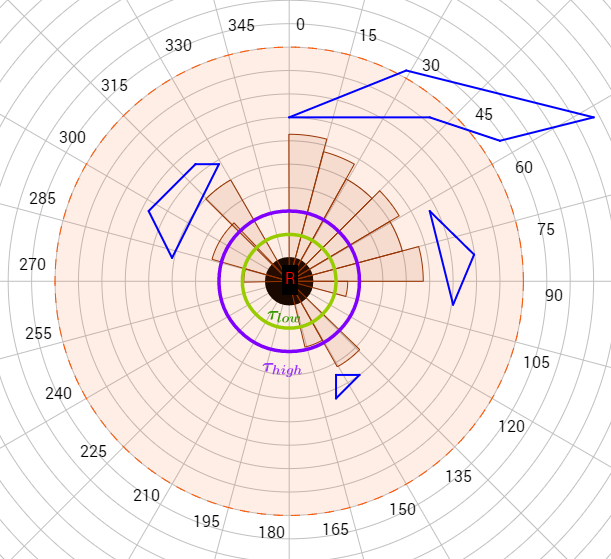
\includegraphics[width=0.9\textwidth]{images/3/polar.png}
\end{figure}
\subsubsection{Binární polární histogram}

Aby bylo možné určit kandidáty pro další směr pohybu, primární histogram musí být převeden do binární podoby.

$$H_{k,i}^{b} = \left\{
\begin{array}{ll}
1&\textrm{jestli $H_{k,i}^p > \tau_{high}$,}\\
0&\textrm{jestli $H_{k,i}^p < \tau_{low}$,}\\
H_{k, i-1}^b&\textrm{jinak.}
\end{array}
\right.
$$

\subsubsection{Výběr kandidátů}

Kandidáty pro nový směr pohybu se volí podle toho, do jaké kategorie je zařazeno volné místo v binárním histogramu. Ty průjezdy, jež mají velikost (tedy vzdálenost mezi pravým okrajem $k_r$ a levým $k_l$) menší, než $s_{max}$, se nazývají úzké, jiné jsou naopak nazývány široké.

Pro úzké průjezdy lze zvolit pouze jednoho kandidáta, a to 

$$\begin{array}{ll}
c_n = \frac{k_r + k_l}{2}&\textrm{centrální sektor}
\end{array}$$

Široké průjezdy mají tři možné kandidáty:

$$\begin{array}{ll}
c_r = k_r + \frac{s_{max}}{2}&\textrm{pravý sektor,}\\

c_l = k_l - \frac{s_{max}}{2}&\textrm{levý sektor,}\\

c_t = k_t&\textrm{pokud $k_t \in \left[c_r;c_l\right]$}
\end{array}$$

Nový směr pohybu se zvolí dle minimální ceny spočítané pro kandidáta $c_i$ pomocí vztahu

\begin{equation}
g(c_i) = \mu_1 \Delta\left(c_i, k_t\right) + \mu_2\Delta\left(c_i, \frac{h}{\alpha}\right) + \mu_3\Delta\left(c_i, k_{d, n-1}\right)
\end{equation}

přičemž $k_{d, n-1}$ je minule zvolený kandidát, 
$\mu_1, \mu_2, \mu_3$ jsou konstanty, zvolené dle vztahu $\mu_1 > \mu_2 + \mu_3$ a také platí, že

\begin{equation}
\Delta(c_1, c_2) = \min\left\{|c_1 - c_2|, |c_1 - c_2 - \frac{360^{\circ}}{\alpha}|, |c_1 - c_2 + \frac{360^{\circ}}{\alpha}|\right\}
\end{equation}


\section{PID regulátor}

%https://www.cs.hmc.edu/~dodds/projects/RobS05/XPort/XPortArticle.pdf
 
Za jízdy je třeba, aby byla mezi robotem a cílem udržována určitá vzdálenost $d$ a hodnota $\phi$ byla co nejmenší, nejlépe nulová. Pro tyto účely je navržen PID regulátor, který pro aktuální odchylku od referenčních bodů spočte dopřednou a úhlovou rychlosti, které se následně převedou na rychlosti motorů. Zjednodušený nákres algoritmu je zobrazen na \ref{pid}.  Pokud $\epsilon_d$, příp. $\epsilon_\phi$, je v pásmu $\left[-\epsilon_{d_0}; \epsilon_{d_0}\right]$, příp. $\left[-\epsilon_{\phi_0}; \epsilon_{\phi_0}\right]$, pak výstup PID regulátoru bude nulový. Jinak se od odchylky odečte hodnota $\epsilon_{d_0}$, příp. $\epsilon_{\phi_0}$, což zaručí to, že se robot nebude kmitat na místě, když bude hodně blízko referenčního bodu a řízení bude plynulé.

\begin{figure}
	\caption{PID regulace}
	
	\label{pid}
	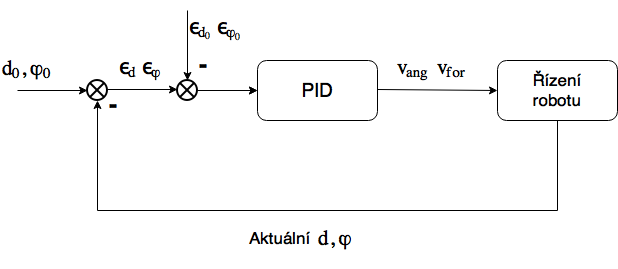
\includegraphics[width=0.9\textwidth, height = 0.4\textwidth]{images/3/PID.png}
\end{figure}


\chapter{Simulace}

%http://www.coppeliarobotics.com/index.html
Pro simulaci byl zvolen V-Rep simulátor. V tomto prostředí byly vytvořeny dva roboty: jeden s vizuální značkou, druhý byl vybaven kamerou a laserovým dálkoměrem a sledoval prvního. Referenční vzdálenost mezi dvěma roboty byla zvolena \SI{1}{\meter}, požadovaná odchylka vizuální značky od středu kamery \SI{0}{\radian}. Maximální dopřední rychlost obou robotů byla nastavena \SI{2.5}{\meter\per\second}

\section{Porovnání algoritmů detekce}

Oba algoritmu byly porovnávány při použití značky o velikosti 10x10 cm a rozlišením kamery 512x512 pixelů. Bylo porovnáno několik parametrů obou algoritmu, a to maximální vzdálenost, na které je vizuální značka ještě detekovatelná, stabilní vzdálenost, při které značka je detekována bez přerušení. Dále se porovnával maximální a stabilní úhel otočení vizuální značky vůči robotu a také průměrný výpočetní čas na jednu iteraci algoritmu. Výsledky jsou znázorněny v tabulce \ref{porovnani}. Je patrné, že detekční schopnosti korelačního algoritmu jsou poněkud horší, než u ArUco detektoru. Avšak je třeba zdůraznit, že sice ArUco detektor dokázal rozpoznat vizuální značku na vzdálenosti přes 5 metrů od kamery, úspěšnost detekcí na tak velké vzdálenosti byla podprůměrná, přibližně 40 \%. Co se týká úhlu otočení značky vůči robotu, tam se korelační algoritmus ukázal být lepší a stabilně detekuje značku při 60$^\circ$ otočení. ArUco má na hranicích detekovatelnosti, tj. při 70$^\circ$ otočení, pouze 15\% úspěšnost.

\begin{table}[hbt]
	\centering
	\caption{Porovnání korelačního algoritmu a ArUco detektoru}
	\label{porovnani}
	\begin{tabular}{|c|c|c|}
		\hline
		Název algoritmu              & Korelační algoritmus & ArUco detektor \\ \hline
		Max. vzdálenost {[}m{]}      & 3.5                 & 5.4           \\ \hline
		Stabilní vzdálenost {[}m{]}  & 3.5                 & 3.8           \\ \hline
		Max. úhel {[}$^\circ${]}     & 60                   & 70             \\ \hline
		Stabilní úhel {[}$^\circ${]} & 60                   & 55             \\ \hline
		Výpočetní doba {[}ms{]}      & 15                   & 15             \\ \hline
	\end{tabular}
\end{table}
Hlavní rozdíl mezi těmito algoritmy spočívá v možnostech jejich využití. Zatímco ArUco detektor je zaměřený pouze na ArUco markery, korelační algoritmus je obecnější a dá se použít fakticky na jakýkoliv typ vizuální značky. ArUco detektor umožňuje přidání dalších značek do své knihovny, ale jedná se pouze o binární obrázky podobné znázorněnému na \ref{aruco_marker}. Korelační algoritmus si poradí i se značkou, kterou nelze reprezentovat jako bit-mapu, viz např. \ref{hiro}.


\begin{figure}
	\caption{Příklad značky pro korelační algoritmus}
	
	\label{hiro}
	
\includegraphics[width=0.5\textwidth]{images/5/r1301.jpg}
\end{figure}

\section{Porovnání naměřených a reálných hodnot}

\begin{figure}[hbt]
	\caption{Poloha sledovaného objektu během simulace}
	
	\label{sled}
	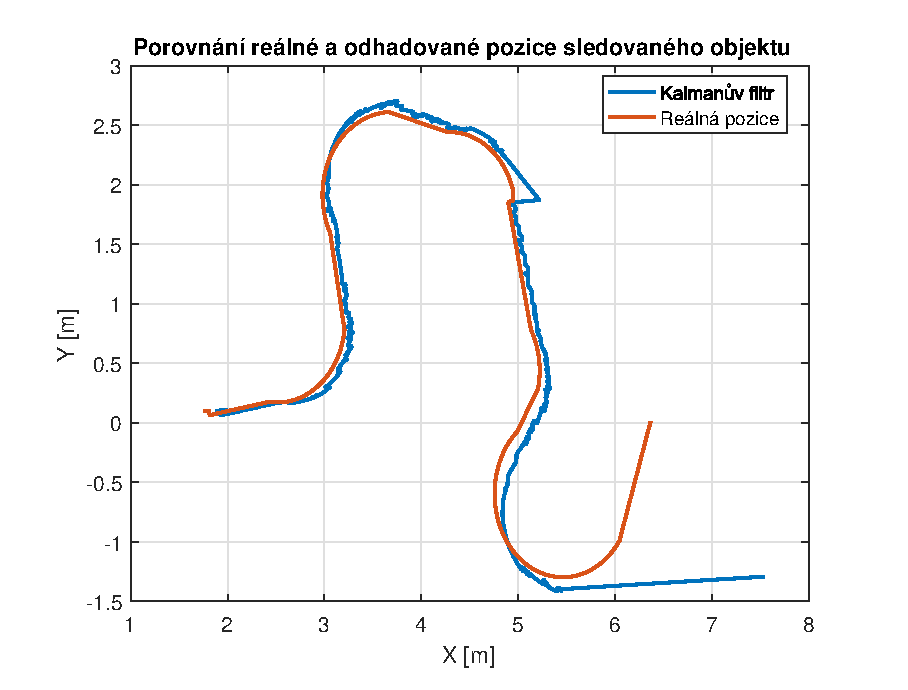
\includegraphics[width=0.9\textwidth]{images/5/pos_pioner.eps}
\end{figure}

Jelikož se v implementovaném programu provádí různá měření, je třeba porovnat, jak naměřené hodnoty jsou správné vůči reálným. Kalmanův filtr, popsaný v \ref{kalman_section}, predikuje polohu cíle a v případě neúspěšné detekce vizuální značky umístění sledovaného objektu vůči robotu je odvozeno právě z predikované polohy. Na obrázku \ref{sled} lze vidět, že výpočet pomocí Kalmanova filtru skoro po celou dobu simulace odpovídá reálné poloze sledovaného objektu. Velká odchylka pak je až na konci simulace, kdy vizuální značka hodně brzo zmizela ze zorného pole robotu a nebylo možné ji v krátké době najít. Toto také odpovídá výsledkům, které jsou na \ref{dist} a \ref{odch}, kde je vidět, že po cca 2000. iteraci je velký rozdíl mezi změřenými a reálnými hodnotami.


\begin{figure}[hbt]
	\caption{Vzdálenost mezi robotem a sledovaným objektem (d)}
	
	\label{dist}
	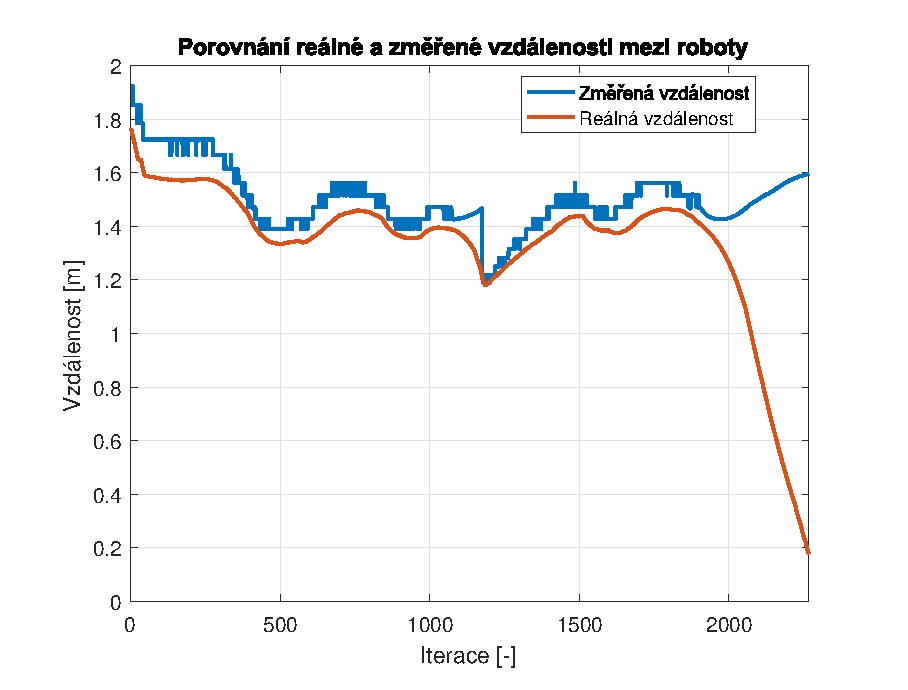
\includegraphics[width=0.9\textwidth]{images/5/dist.eps}
\end{figure}


\begin{figure}[hbt]
	\caption{Odchylka sledovaného objektu od středu kamery $\phi$}
	
	\label{odch}
	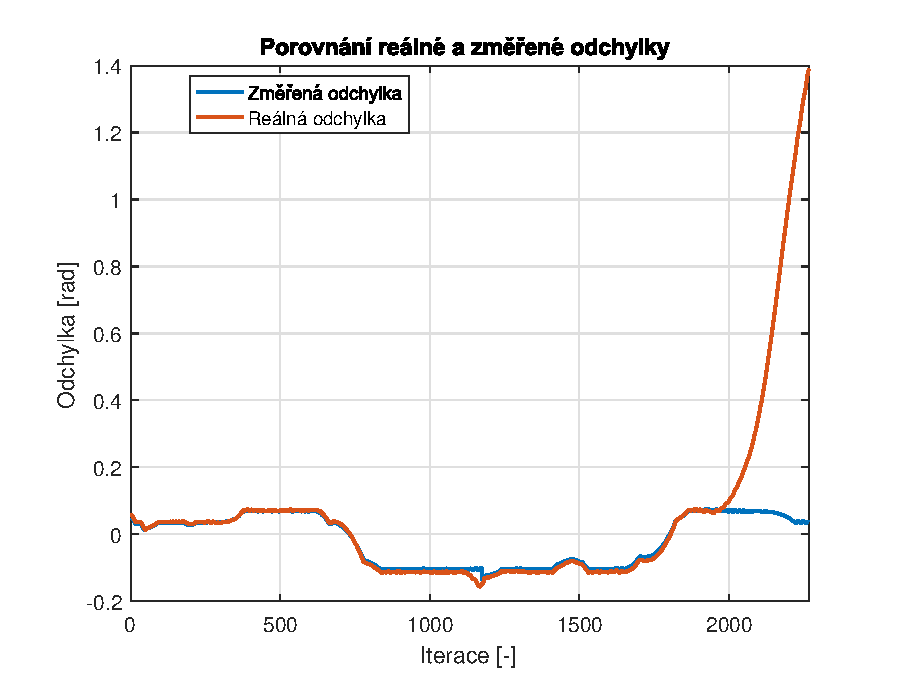
\includegraphics[width=0.9\textwidth]{images/5/odchylka.eps}
\end{figure}
Na obrázku \ref{dist} je také vidět, že změřená vzdálenost není stejná, jako reálná. Je to způsobeno nepřesnou kalibrací referenční vzdálenosti mezi následovaným a sledujícím roboty. Kdyby kalibrace byla přesnější, bylo by možné dosáhnout podobného výsledku, jako pro odchylku od středu kamery (viz \ref{odch}), kde měření odpovídá reálné hodnotě.

\section{Měření polohy robotu}

\begin{figure}
	\caption{Poloha robotu během simulace}
	
	\label{rob_pos}
	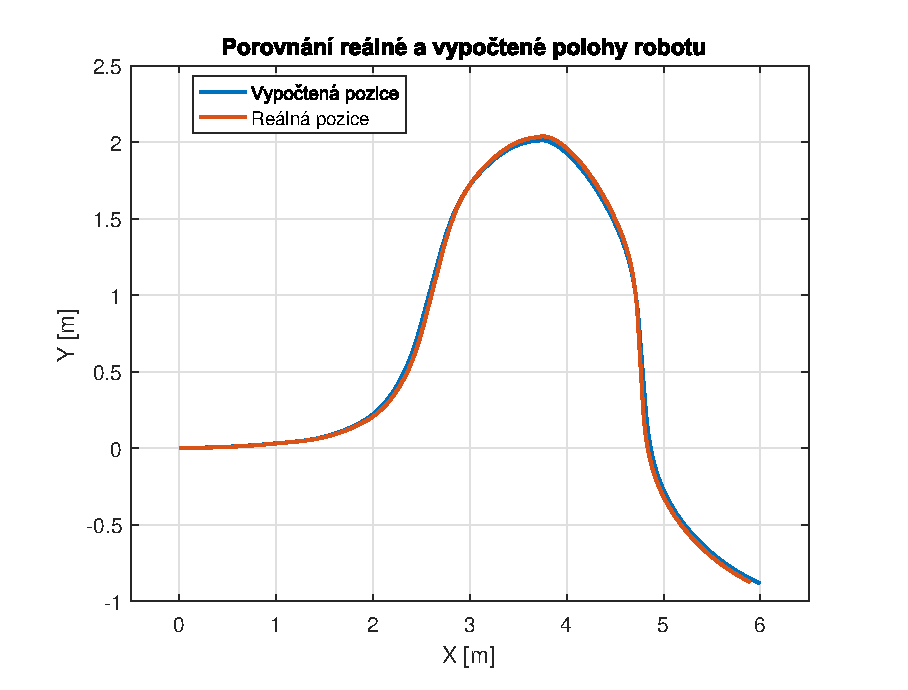
\includegraphics[width=0.9\textwidth]{images/5/pos_rob.eps}
\end{figure}

%https://chess.eecs.berkeley.edu/eecs149/documentation/differentialDrive.pdf
Jak bylo řečeno v \ref{kalman_section}, aby bylo možné spočítat polohu cíle vůči robotu, je třeba znát polohu robotu v globálních souřadnicích. Ačkoliv V-Rep simulátor nabízí možnosti pro přesné měření polohy objektů ve světových souřadnicích, v reálném světě tato možnost nemusí být použitelná, protože např. při navigaci robotu uvnitř budov nelze použít GPS. Proto v sekci \ref{ss_section} byl zaveden souřadnicový systém, ve kterém se poloha robotu počítá. Pro toto měření v simulátoru lze odečítat vnitřní polohu rotačních kloubu robotu, na které jsou přidělány kola. V případě robotu s diferenciálním řízením, jeho pozici lze spočítat jako

\begin{equation}
\begin{bmatrix}
x\\
y\\
h
\end{bmatrix} = 
\begin{bmatrix}
x + \frac{(\Delta R + \Delta L)r_{k}}{2}\cos(h)\\
y + \frac{(\Delta R + \Delta L)r_{k}}{2}\sin(h)\\
h + \frac{(\Delta R - \Delta L)r_k}{2r_r}
\end{bmatrix},
\end{equation}

přičemž  $\Delta L$ a $\Delta R$ značí změnu vnitřní polohy levého a pravého kloubů za čas $\Delta t$, $r_k$ je poloměr kola a $r_r$ je poloměr robotu, neboli polovina vzdálenosti mezi koly.

Porovnání reálné, tj. změřené v simulátoru, a vypočtené polohy robotu ve zvoleném souřadnicovém systému lze vidět na obrázku \ref{rob_pos}. Je patrné, že pro použitý typ robotu výpočet je hodně přesný a při použití přesných enkodérů lze tento výpočet aplikovat i na reálném robotu.

\section{Trajektorie robotů}


\begin{figure}
	\caption{Trajektorie robotu a sledovaného objektu}
	
	\label{trajektorie}
	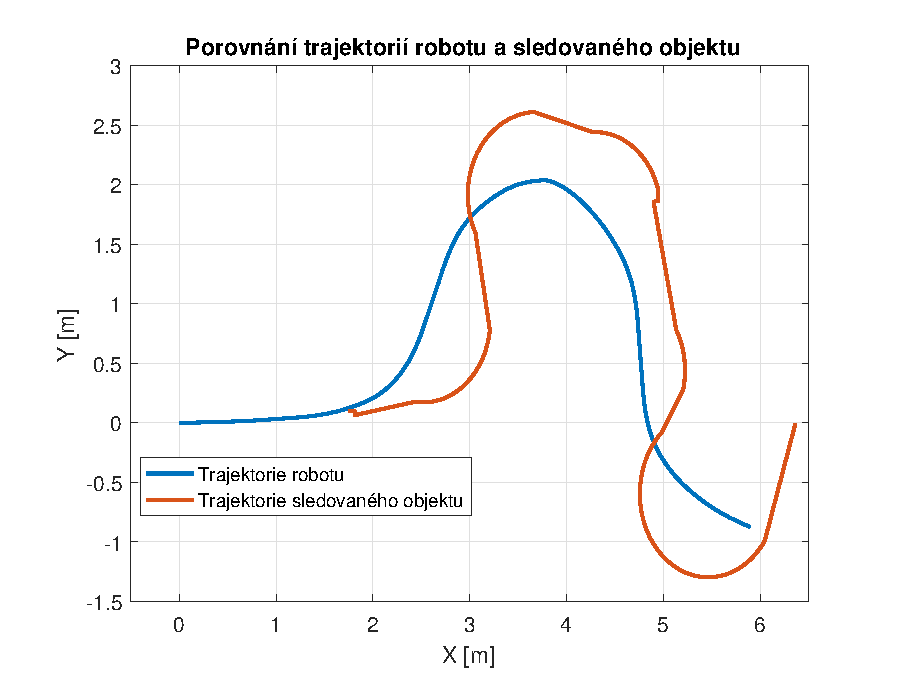
\includegraphics[width=0.9\textwidth]{images/5/trajektorie.eps}
\end{figure}
\chapter{Závěr}
\appendix

\printindex

%\bibliographystyle{amsalpha}
%\bibliography{ctutest}

\end{document}